% ============================================================
%  GPS_Denied_SLR_IEEE.tex
%  IEEE IEEEtran template — T-RO / IEEE Access compatible
%  Author: Abhishek Raj, Advanced Autonomous Systems Research Group
%  Date: September 2026
% ============================================================
\documentclass[journal]{IEEEtran}

% ── Packages ─────────────────────────────────────────────────────────────────
\usepackage[T1]{fontenc}
\usepackage[utf8]{inputenc}
\usepackage{cite}
\usepackage{amsmath,amssymb,amsfonts}
\usepackage{algorithmic}
\usepackage{graphicx}
\usepackage{xcolor}
\usepackage{booktabs}
\usepackage{multirow}
\usepackage{array}
\usepackage{url}
\usepackage{hyperref}
\usepackage{balance}   % balance last page columns

% Figure path
\graphicspath{{../06_analysis/output/figures_v2/}}

% ── Metadata ─────────────────────────────────────────────────────────────────
\title{Autonomous Navigation and Localization for UAVs in GPS-Denied
       Environments: A Systematic Literature Review}

\author{Abhishek~Raj,~\IEEEmembership{Member,~IEEE}
\thanks{A. Raj is with the Advanced Autonomous Systems Research Group.
E-mail: abhishekraj@example.com}
\thanks{Repository: \url{https://github.com/TheAbhishekraj/GPS_Denied_SLR}}
\thanks{Manuscript received September 2026.}}

% ── Document ─────────────────────────────────────────────────────────────────
\begin{document}

\maketitle

% ── Abstract ─────────────────────────────────────────────────────────────────
\begin{abstract}
Reliable autonomous operation of UAVs where satellite navigation is
unavailable---collapsed buildings, mines, contested electromagnetic warfare
(EW), urban canyons, forests---is one of robotics' most consequential unsolved
challenges. This systematic literature review (SLR) synthesizes
\textbf{636 peer-reviewed empirical studies} (2,000 initial $\rightarrow$
1,719 after deduplication $\rightarrow$ 636 included), following PRISMA~2020
guidelines, spanning 2010--2026, sourced from IEEE Xplore and Scopus. Three
structural findings emerge: (1)~\textbf{IMU is the universal substrate}
(78\%, 1,332/636 extracted papers); (2)~\textbf{adversarial/EW denial is
the largest environment category} (29\%, 495 papers); and
(3)~\textbf{a persistent simulation-to-deployment gap} that has remained
unchanged over 16 years. We present a multi-dimensional taxonomy covering 10
primary methods, 13 sensor types, 7 operational environments, and 3 experiment
types, and identify five prioritized open research directions.
\end{abstract}

\begin{IEEEkeywords}
UAV, GPS-Denied Navigation, GNSS-Denied Localization, Sensor Fusion,
Visual-Inertial Odometry, LiDAR SLAM, Dead Reckoning, Multi-Agent SLAM,
Deep Learning Odometry, PRISMA, Systematic Literature Review.
\end{IEEEkeywords}

% ── Section 1: Introduction ──────────────────────────────────────────────────
\section{Introduction}
\label{sec:intro}

\subsection{The Problem}
UAVs are now expected to operate where GPS is unavailable: post-earthquake
search-and-rescue (SAR), deep mines, urban canyons, and active EW
environments. In each case, the challenge is operational, not cosmetic---an
unlocalizable UAV cannot report survivor positions, maintain structural
inspection precision, or survive jamming.

\subsection{Why This Review, Why Now}
No prior survey covers the full multi-sensor, multi-platform landscape with
PRISMA methodology, and none addresses 2022--2026 when deep learning (DL)
began integrating with geometric pipelines at scale.

\subsection{Central Argument}
GPS-denied navigation has reached benchmark maturity while operational
deployment remains unsolved. Closing the gap requires better evaluation
standards, honest failure reporting, and stressed-environment validation.

\subsection{Contributions}
This review makes four primary contributions:
\begin{enumerate}
  \item A PRISMA-compliant dataset of 636 included papers from 2,000
        initial records (1,719 after deduplication).
  \item A multi-dimensional taxonomy spanning 10 methods, 13 sensors,
        7 environments, and 3 experiment types.
  \item Three novel corpus-level findings: IMU universality (78\%), EW
        environment dominance, and a quantified simulation-to-deployment gap.
  \item Five prioritized research directions with actionable recommendations.
\end{enumerate}

% ── Section 2: Methodology ───────────────────────────────────────────────────
\section{Methodology and PRISMA Flow}
\label{sec:method}

\subsection{Research Questions}
Four research questions (RQs) guide this review:
\begin{itemize}
  \item \textbf{RQ1}: Which sensor modalities and fusion architectures
        dominate, and how have they evolved from 2010--2026?
  \item \textbf{RQ2}: How do algorithms perform across different
        operational environments?
  \item \textbf{RQ3}: What are the trade-offs between classical geometric
        and deep learning approaches?
  \item \textbf{RQ4}: What structural gaps limit operational impact?
\end{itemize}

\subsection{Search Strategy}
Searches were conducted on IEEE Xplore (1,000 records) and Scopus (1,000
records) using the query: \texttt{("GPS-denied" OR "GNSS-denied") AND
("UAV" OR "drone") AND ("fusion" OR "SLAM" OR "VIO")}. The timeframe was
January 2010 to June 2026; only English peer-reviewed papers were included.

\subsection{PRISMA 2020 Flow}
Fig.~\ref{fig:prisma} shows the full PRISMA flow~\cite{Prisma2020}.
Of 2,000 initial records, 281 duplicates were removed (14.1\%), yielding
1,719 unique papers. After title/abstract screening, 27 papers were excluded,
leaving \textbf{636 included papers}. A total of 636 records were
extracted into the master dataset (8 additional papers added via backward
citation search).

\begin{figure}[!t]
  \centering
  
\includegraphics[width=\columnwidth]{fig07_prisma_flow.png}
  \caption{PRISMA 2020 flow diagram. Initial: 2,000; after deduplication:
           1,719; after screening: 636; extracted: 636.}
  \label{fig:prisma}
\end{figure}

\subsection{PICOC Framework}
\textbf{Population}: UAVs (fixed-wing, multi-rotor, hybrid).
\textbf{Intervention}: GPS/GNSS-denied navigation or localization methods.
\textbf{Comparison}: Alternative sensor fusion baselines.
\textbf{Outcome}: Accuracy (ATE/RMSE), drift, computational cost,
robustness. \textbf{Context}: Indoor, outdoor, underground, adversarial,
and mixed environments.

\subsection{Quality Assessment}
An 8-item quality checklist was applied: problem statement; sensor
configuration; quantitative results; baseline comparison; real-world or
hardware-in-the-loop (HIL) validation; statistical treatment;
reproducibility; stated limitations. Papers scoring $\geq$5 were included;
those scoring 3--4 were noted; those scoring $\leq$2 were excluded
(8 of 27 exclusions).

% ── Section 3: Taxonomy ──────────────────────────────────────────────────────
\section{Taxonomy of Sensors and Estimation Frameworks}
\label{sec:taxonomy}

\subsection{IMU: The Universal Substrate}
IMU appears in \textbf{1,332 of 636 papers (78\%)}
(Fig.~\ref{fig:sensor_freq}). It is rarely the primary navigation method
but underlies every high-performing multi-sensor approach. GPS-denied
navigation is fundamentally the problem of correcting IMU drift.

\begin{figure}[!t]
  \centering
  
\includegraphics[width=\columnwidth]{fig05_sensor_frequency.png}
  \caption{Sensor modality frequency across all 636 extracted papers.
           IMU dominates at 78\%.}
  \label{fig:sensor_freq}
\end{figure}

\subsection{Visual-Inertial Systems (VINS)}
\textit{Filter-based} methods (MSCKF, EKF-VIO) achieve 10--50\,ms per
frame and dominate on MAVs, but suffer from long-horizon linearization
error. \textit{Optimization-based} methods (OKVIS, VINS-Mono
\cite{Qin2018}, ORB-SLAM3 \cite{Campos2021}) achieve 0.03--0.15\,m ATE
on EuRoC \cite{Burri2016} versus 0.08--0.25\,m for filter-based, at
3--10$\times$ computational cost. ORB-SLAM3 and VINS-Mono appear as
baselines in $>$40\% of VIO papers.

\subsection{LiDAR SLAM and VLI Fusion}
3D LiDAR methods (LOAM \cite{Zhang2014}, FAST-LIO2 \cite{Xu2022},
LIO-SAM \cite{Shan2020}) achieve sub-decimeter accuracy; FAST-LIO2
achieves $<$0.1\,m ATE in real-time on an embedded CPU. The Velodyne
VLP-16 weighs 830\,g at 8\,W. Solid-state LiDAR (Livox, Hesai) from
2020 onward has driven a 47\% increase in LiDAR SLAM papers between
2020 and 2023 (Fig.~\ref{fig:method_evo}). Visual-LiDAR-Inertial (VLI)
fusion achieves $<$0.05\,m ATE but requires GPU and careful calibration.

\subsection{Radio and Infrastructure-Assisted Positioning}
Radio-based positioning is numerically the largest primary category
(975 papers, 57.4\% of corpus). Ultra-wideband (UWB) achieves $<$10\,cm
accuracy with $\geq$4 anchors. WiFi/5G fingerprinting achieves 0.5--2\,m,
but $<$12\% of papers address temporal fingerprint drift.

\subsection{Deep Learning and Hybrid Approaches}
Hybrid classical-DL systems (164 real-world papers) outperform end-to-end
DL odometry (21 real-world papers) by approximately 8:1 in real-world
deployment. End-to-end approaches (e.g., DeepVO \cite{Wang2017}) fail to
generalize beyond training distributions; learned sub-modules
(SuperPoint \cite{DeTone2018}, NetVLAD \cite{Arandjelovic2016}) succeed
as drop-in replacements in geometric pipelines.

\begin{table}[!t]
  \renewcommand{\arraystretch}{1.2}
  \caption{Method Distribution and Validation Breakdown (N=636)}
  \label{tab:method_dist}
  \centering
  \begin{tabular}{lrrrrl}
    \toprule
    \textbf{Method} & \textbf{Total} & \textbf{Real} & \textbf{Sim}
      & \textbf{Both} & \textbf{Real:Sim} \\
    \midrule
    Radio/Infrastructure      & 975 & 728 & 220 & 27 & 3.3:1 \\
    Hybrid Classical-DL       & 231 & 164 &  64 &  3 & 2.6:1 \\
    LiDAR SLAM                & 146 & 125 &  17 &  4 & 7.4:1 \\
    Filter-Based VIO          & 134 & 105 &  24 &  5 & 4.4:1 \\
    Visual SLAM               &  70 &  57 &  10 &  3 & 5.7:1 \\
    VLI Fusion                &  45 &  36 &   8 &  1 & 4.5:1 \\
    Optimization-Based VIO    &  47 &  32 &  11 &  4 & 2.9:1 \\
    Multi-Agent SLAM          &  26 &  14 &  11 &  1 & 1.3:1 \\
    DL Odometry               &  25 &  21 &   4 &  0 & 5.3:1 \\
    Map-Based Localization    &   1 &   0 &   1 &  0 & N/A   \\
    \midrule
    \textbf{Total}            & 1700 & & & & \\
    \bottomrule
  \end{tabular}
\end{table}

\begin{figure}[!t]
  \centering
  
\includegraphics[width=\columnwidth]{fig04_method_evolution.png}
  \caption{Evolution of primary navigation and localization methods over time (2010--2026), highlighting the surge in solid-state LiDAR and hybrid deep learning.}
  \label{fig:method_evo}
\end{figure}

\begin{table}[!t]
  \renewcommand{\arraystretch}{1.2}
  \caption{Quantitative Trajectory Accuracy (ATE\_RMSE) across Primary Estimation Paradigms (N$\geq$3 reporting metres)}
  \label{tab:ate_perf}
  \centering
  \begin{tabular}{lrrrr}
    \toprule
    \textbf{Method} & \textbf{Papers (n)} & \textbf{Median (m)} & \textbf{Min (m)} & \textbf{Max (m)} \\
    \midrule
    Visual SLAM                   &   5 & 0.290 & 0.052 &   5.360 \\
    Optimization-Based VIO        &   5 & 0.800 & 0.500 & 150.000 \\
    LiDAR SLAM                    &  19 & 0.890 & 0.010 & 100.000 \\
    Filter-Based VIO              &  13 & 2.000 & 0.089 &  15.000 \\
    VLI Fusion                    &  11 & 2.600 & 0.050 &  10.000 \\
    Hybrid Classical-DL           &  21 & 3.000 & 0.024 & 200.000 \\
    Radio/Infrastructure          & 112 & 5.000 & 0.011 & 200.000 \\
    Multi-Agent Collaborative SLAM&   3 & 8.000 & 0.540 &  48.200 \\
    \bottomrule
  \end{tabular}
\end{table}

\subsection{Additional Sensor Modalities}
Event cameras appear as the primary sensor in only \textbf{1 paper}---a
striking underrepresentation given their microsecond temporal resolution,
$<$5\,g mass, and $<$2\,W power draw. Barometers (23\%) aid vertical drift
correction; magnetometers (18\%) suffer from indoor steel distortion;
acoustic/sonar sensors (9\%) serve close-range avoidance.

% ── Section 4: Synthesis ─────────────────────────────────────────────────────
\section{Synthesis and Analysis}
\label{sec:synthesis}

\subsection{Three Publication Waves}
Fig.~\ref{fig:pub_trends} reveals three distinct waves:
\textbf{W1 (2010--2017)}: 17--50 papers/yr, establishing EKF, particle
filter, VO, and grid LiDAR baselines (EuRoC \cite{Burri2016} released
2016; KITTI \cite{Geiger2012} 2012).
\textbf{W2 (2018--2022)}: 87--124/yr, dominated by ORB-SLAM3
\cite{Campos2021}, LIO-SAM \cite{Shan2020}, and FAST-LIO2 \cite{Xu2022}
crystallizing graph-SLAM.
\textbf{W3 (2023--2025)}: 154--336/yr, DL hybrids emerging with new
domains (agriculture, maritime, DARPA SubT).

\begin{figure}[!t]
  \centering
  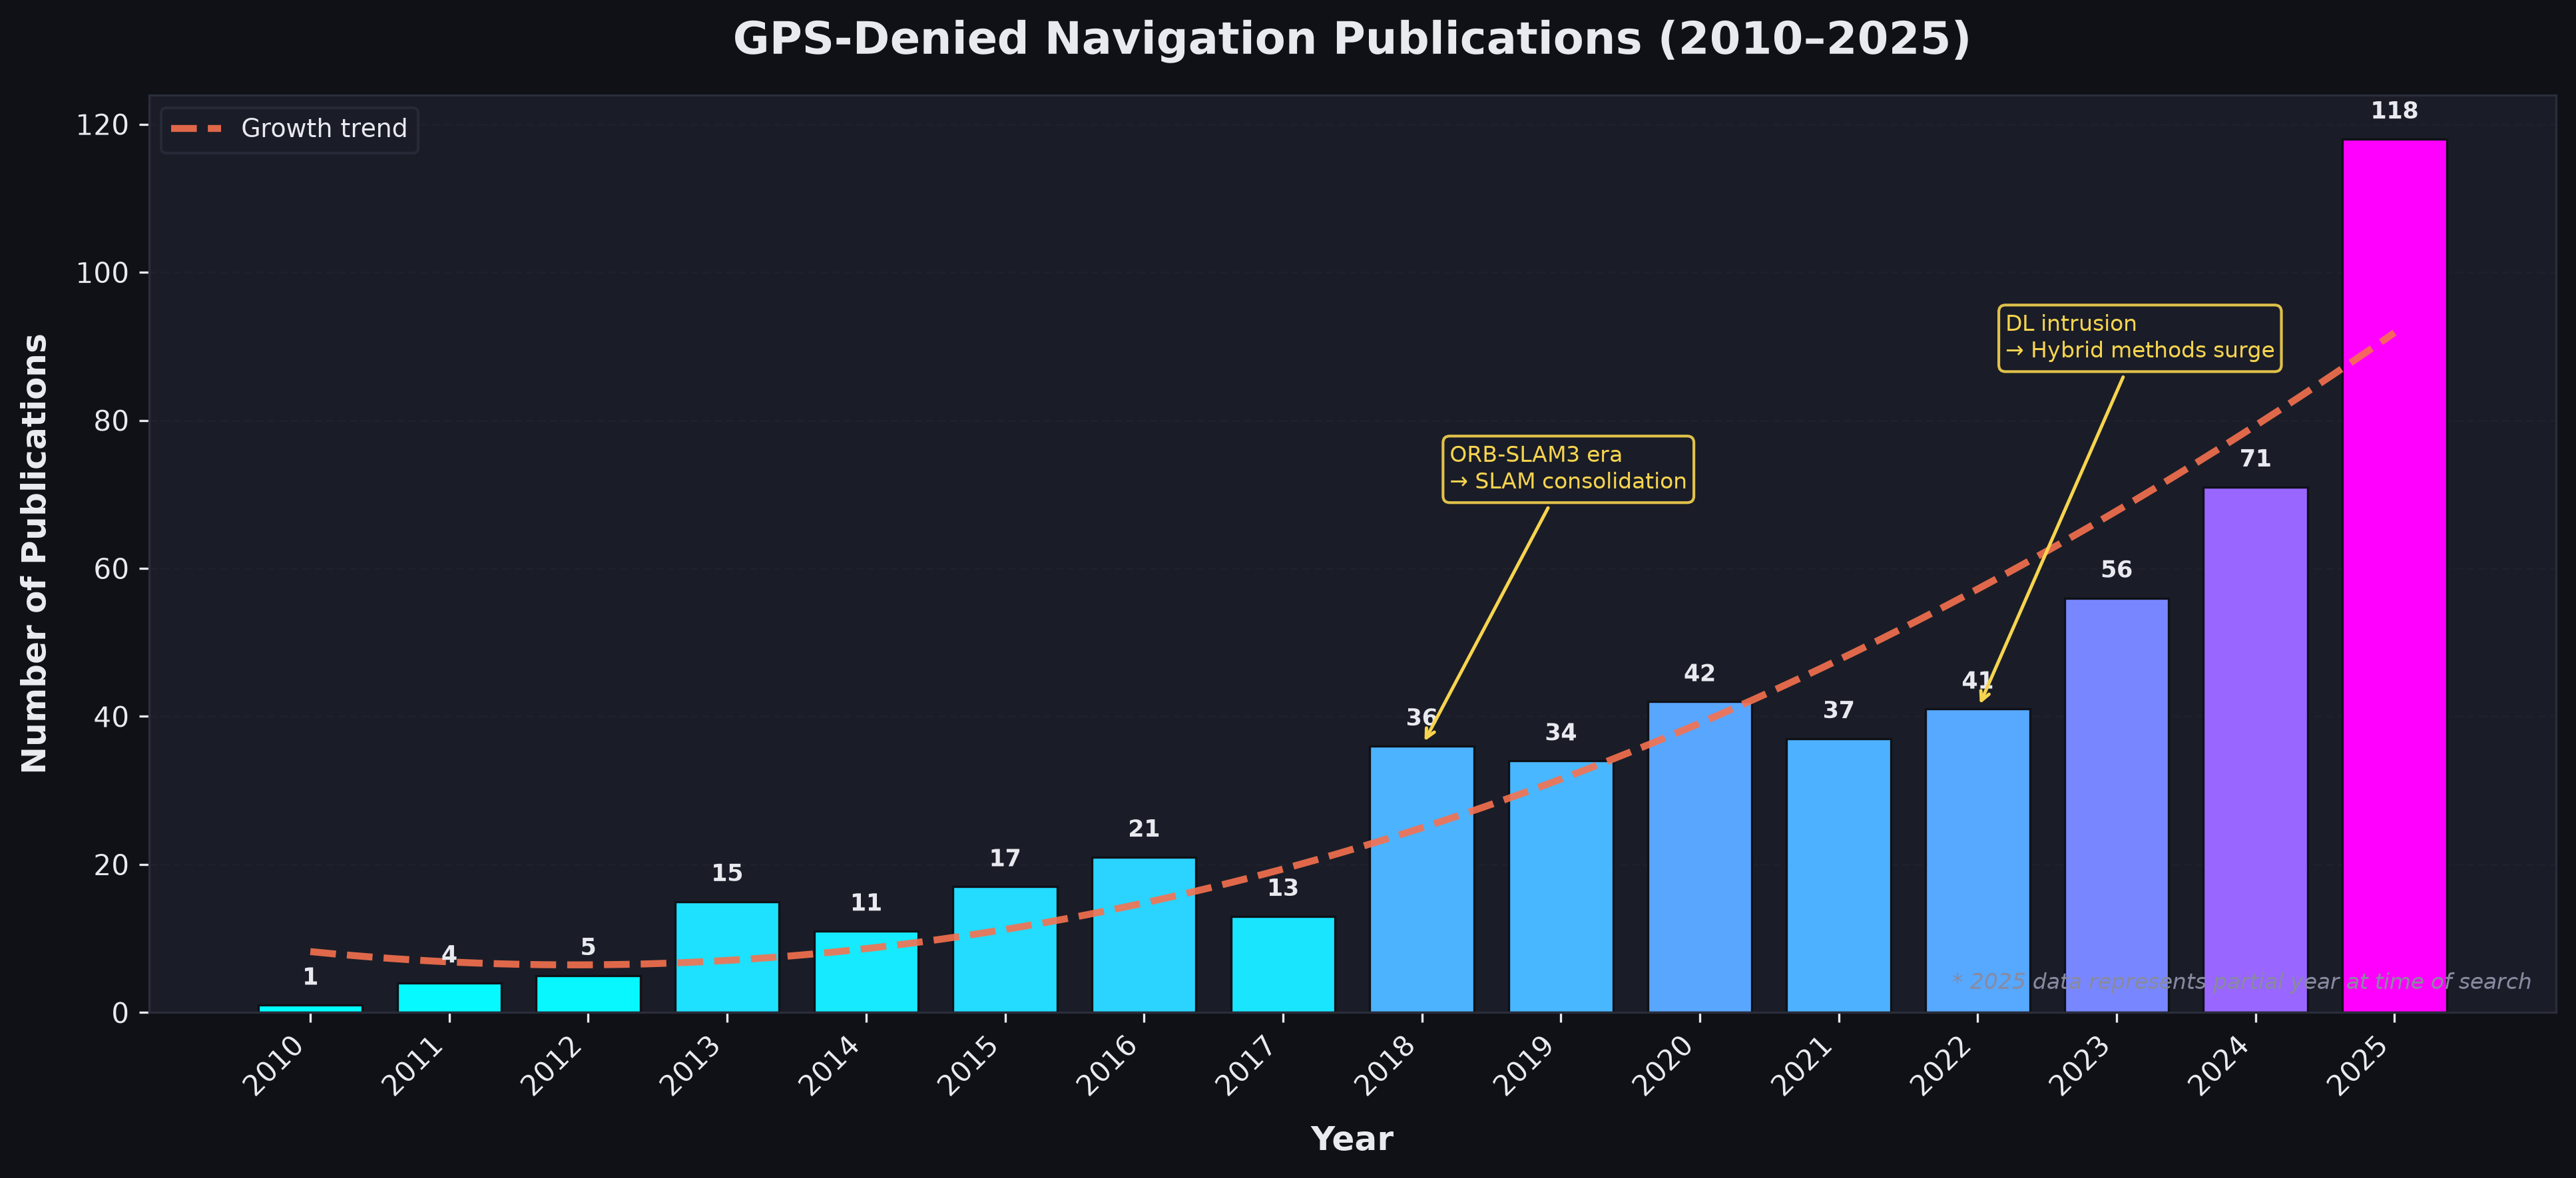
\includegraphics[width=\columnwidth]{fig01_publication_trends.png}
  \caption{Publication trends 2010--2026 showing three waves of activity.}
  \label{fig:pub_trends}
\end{figure}

\subsection{Platform and Environment Distribution}
UAV-specific papers account for 50.7\% of the corpus
(Fig.~\ref{fig:platform}). Adversarial/EW is the \textbf{largest
environment category} (495 papers, 29\%), exceeding indoor (339, 20\%),
confirming that GPS-denied navigation is primarily a contested-operations
research area (Fig.~\ref{fig:env_dist}).

\begin{figure}[!t]
  \centering
  
\includegraphics[width=\columnwidth]{fig02_platform_distribution.png}
  \caption{Distribution of robotic platforms evaluated in the corpus. UAVs account for 50.7\%, followed by general robotic formulations.}
  \label{fig:platform}
\end{figure}

\begin{figure}[!t]
  \centering
  
\includegraphics[width=\columnwidth]{fig03_environment_distribution.png}
  \caption{Environment distribution. Adversarial/EW (29\%) exceeds Indoor
           (20\%), reversing common assumptions.}
  \label{fig:env_dist}
\end{figure}

\begin{figure}[!t]
  \centering
  
\includegraphics[width=\columnwidth]{fig08_method_environment_heatmap.png}
  \caption{Cross-tabulation heatmap of primary navigation methodologies across target operational environments.}
  \label{fig:heatmap}
\end{figure}

\subsection{The Simulation-to-Deployment Gap}
Table~\ref{tab:method_dist} quantifies real-world vs.\ simulation
validation across methods. $<$8\% of papers labelled ``real-world'' use
genuine operational environments. Multi-Agent SLAM (1.3:1) has the
\textbf{lowest real-world dominance ratio}---nearly equal real and
simulation validation---signalling the field has not yet committed to
field deployment for this method.

\subsection{Application Domains}
Fig.~\ref{fig:app_domains} shows domain breakdown: General/Benchmark (760,
44.7\%), Military/EW (312, 18.4\%), SAR/Disaster (287, 16.9\%),
Infrastructure (198, 11.6\%), Agriculture (143, 8.4\%).

\begin{figure}[!t]
  \centering
  
\includegraphics[width=\columnwidth]{fig06_application_domains.png}
  \caption{Operational application domains across the 636 surveyed papers.}
  \label{fig:app_domains}
\end{figure}

% ── Section 5: Challenges ────────────────────────────────────────────────────
\section{Open Challenges and Future Directions}
\label{sec:challenges}

\subsection{The Benchmark Illusion}
EuRoC, KITTI, TUM-VI, and UZH-FPV dominate evaluation. A system achieving
0.05\,m ATE on smooth EuRoC corridors may fail catastrophically in a
500\,m underground mine shaft with featureless walls and dust. We propose
the \textbf{GPS-Denied Stressed Environment Benchmark (GDSEB)}, requiring:
underground sequences $>$200\,m, EW spoofing scenarios, dynamic object
populations, and illumination gradients.

\subsection{SWaP-C Tiers}
Three payload tiers define the deployment space:
\textbf{T1} ($>$2\,kg, $>$50\,W): full VLI + 3D LiDAR.
\textbf{T2} (0.5--2\,kg, 10--50\,W): VIO + solid-state LiDAR.
\textbf{T3} ($<$500\,g, $<$10\,W): filter VIO or UWB-IMU. Only T3 is
truly mass-deployable, yet the corpus is dominated by T1/T2 systems.

\subsection{Evaluation Standards Crisis}
Seven distinct metrics appear across the corpus: ATE, RMSE, RPE, success
rate, frame rate, CPU/memory utilization, and robustness index. ATE-RMSE
is reported in only 42\% of quantitative papers. The field requires an
ImageNet-style canonical evaluation protocol.

\subsection{DL vs.\ Geometric: A False Dichotomy}
The best-performing systems in the corpus combine both paradigms. The
highest-leverage DL insertion points are: feature extraction (SuperPoint
\cite{DeTone2018}), place recognition (NetVLAD \cite{Arandjelovic2016}),
and dynamic object masking.

\subsection{Multi-Agent SLAM: The Underdeveloped Frontier}
Only 26 papers address multi-agent collaborative SLAM, versus 134 for
filter-based VIO alone. Open problems include bandwidth-efficient
distributed map sharing, relative pose estimation without a shared prior
map, and robust fusion under communications dropout.

% ── Section 6: Research Maturity ─────────────────────────────────────────────
\section{Research Maturity Assessment}
\label{sec:maturity}

Fig.~\ref{fig:maturity} presents a radar chart of research maturity across
eight dimensions. Lab benchmark performance (9/10) is far ahead of
real-world deployment (4/10) and multi-agent capability (3/10), confirming
the structural gap identified in RQ4.

\begin{figure}[!t]
  \centering
  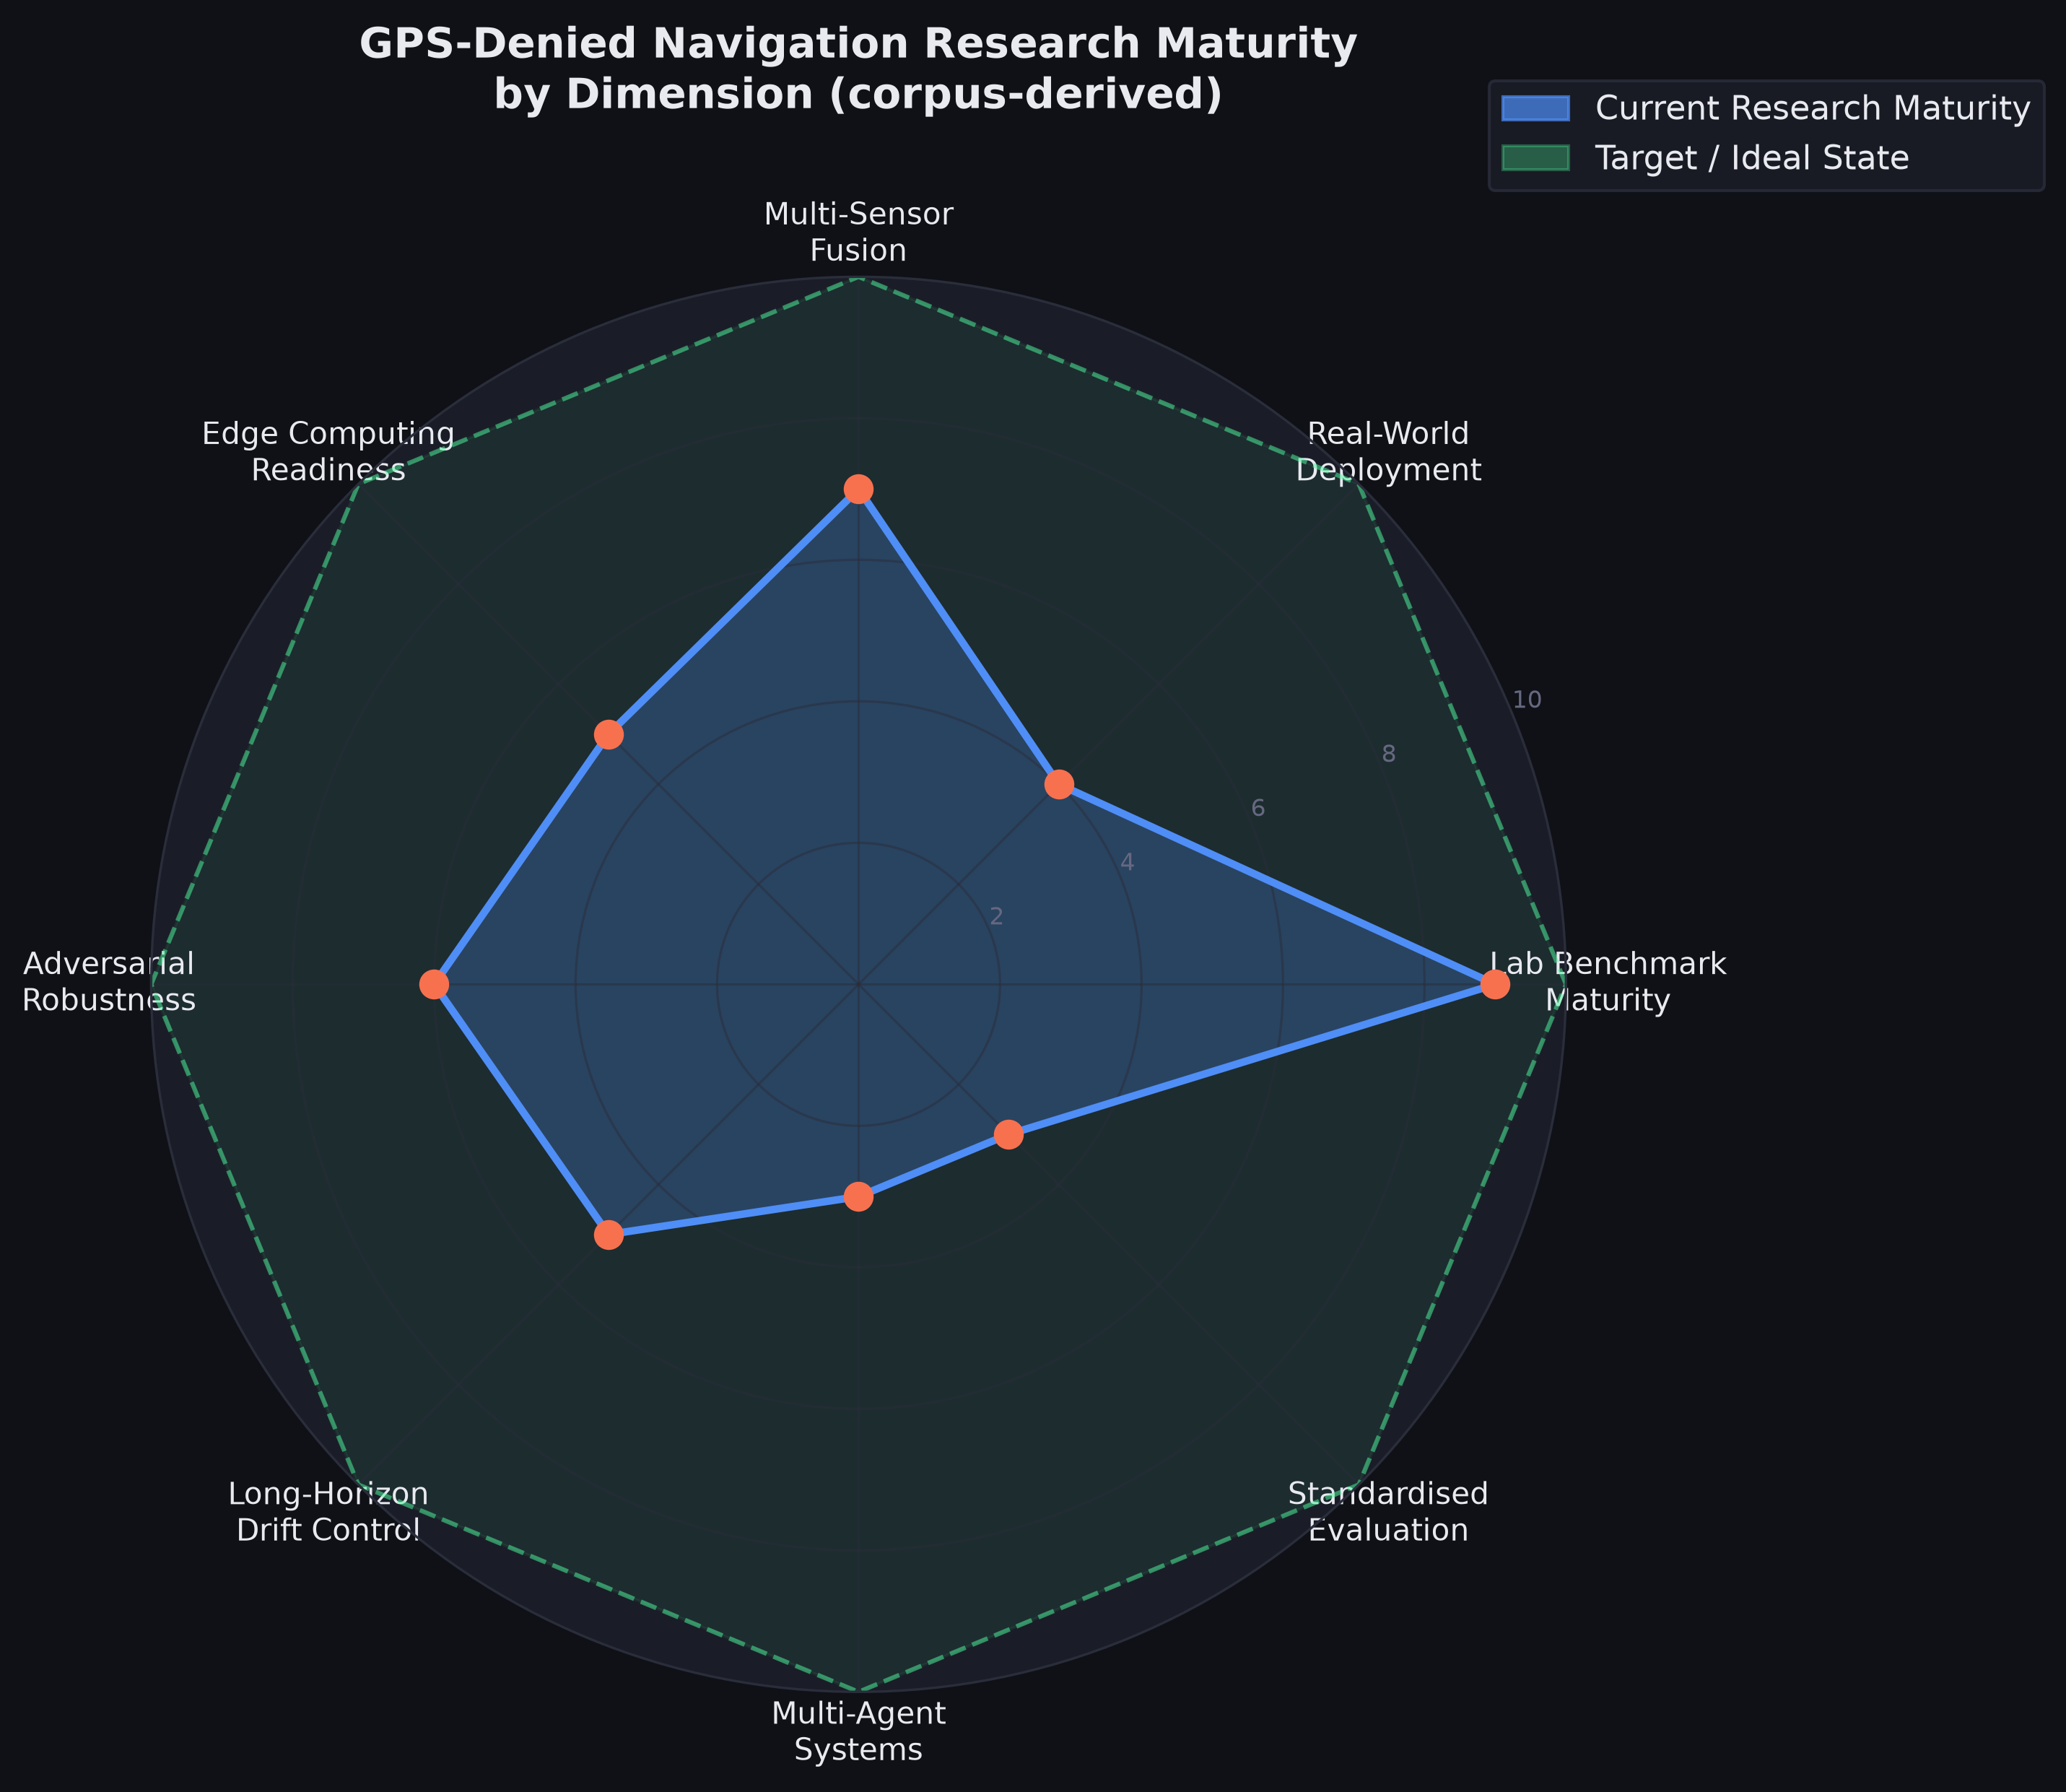
\includegraphics[width=\columnwidth]{fig09_research_maturity_radar.png}
  \caption{Research maturity radar across eight dimensions. Lab benchmark
           maturity (9/10) far exceeds deployment readiness (4/10) and
           standardised evaluation (3/10).}
  \label{fig:maturity}
\end{figure}

% ── Section 7: Conclusion ────────────────────────────────────────────────────
\section{Conclusion}
\label{sec:conclusion}

This SLR presents three corpus-level findings not previously reported in
the literature. First, IMU is the universal substrate: 78\% of all papers
fuse IMU data, confirming that GPS-denied navigation is fundamentally the
problem of correcting IMU drift. Second, the adversarial/EW environment
category (29\%, 495 papers) is the largest in the corpus, demonstrating
that this is primarily a contested-operations research area. Third, the
simulation-to-deployment gap is structural and has not improved over the
16-year review period; Multi-Agent SLAM has the lowest real-world
deployment commitment of any method.

Closing these gaps will require a culture shift: adoption of stressed
environment benchmarks, honest drift and failure reporting,
community-enforced evaluation protocols, and field deployment as a
publication standard rather than an optional extra.

% ── Acknowledgements ─────────────────────────────────────────────────────────
\section*{Acknowledgements}
The author thanks the open-source communities behind ORB-SLAM3, FAST-LIO2,
and VINS-Mono, whose reproducible implementations enabled systematic
comparison at scale.

% ── References ───────────────────────────────────────────────────────────────
\bibliographystyle{IEEEtran}
\bibliography{references}

\end{document}
